\begin{frame}{CVC/BVCによるNC検出器群のオーバーキル}
  \label{page:effNC}
  
  \begin{tabular}{cc}
    \begin{minipage}{0.5\hsize}
      \begin{figure}
        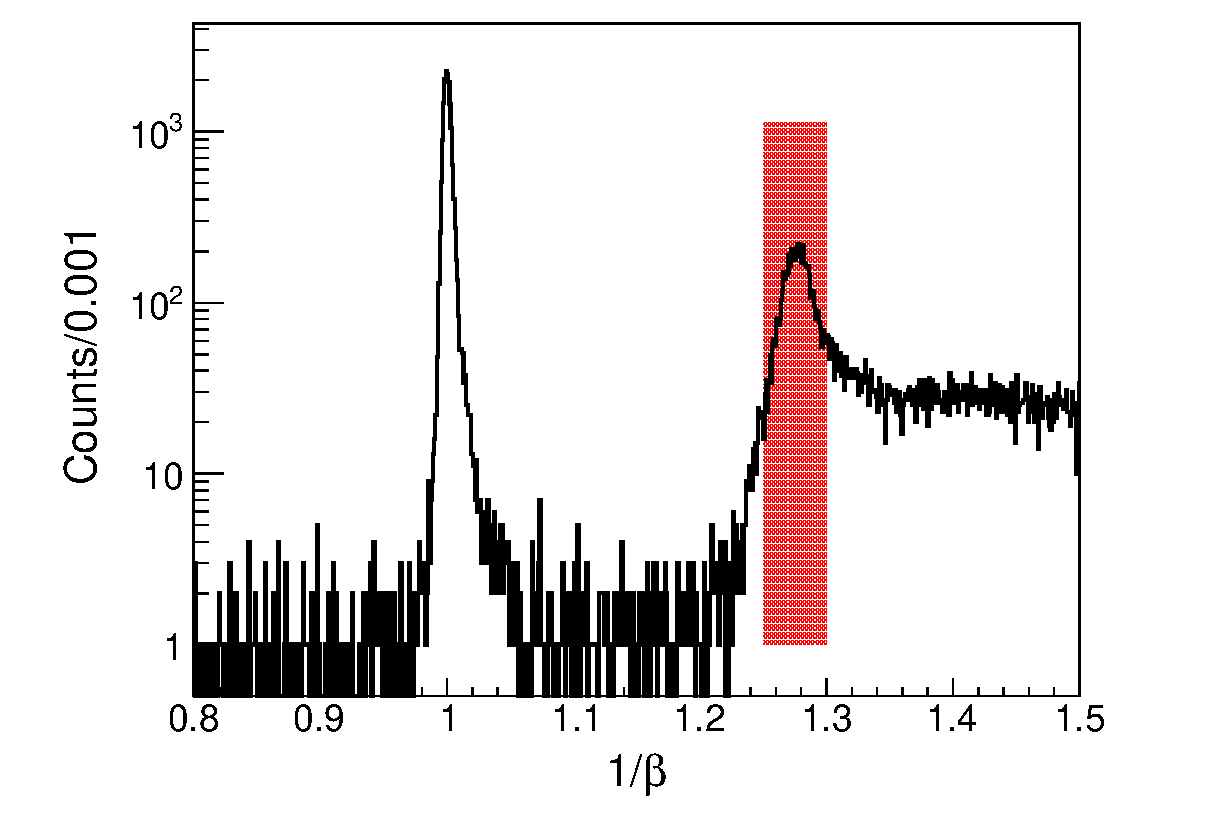
\includegraphics[width=6.5cm]{../pic/Run78//NC/NC_overkill_trig.eps}
      \end{figure}
    \end{minipage}
    \begin{minipage}{0.5\hsize}
      \scriptsize
      $Neutral$トリガー以外で取得されたイベントを使い、
      NC レイヤー1を荷電粒子のベトカウンターに使う。\\
      NC レイヤー$2 \sim 7$で$1/\beta$を測定し(右図)、\\
      赤領域を純弾性散乱イベントとして母数イベントとする。
    \end{minipage}
  \end{tabular}
  \centering
  (CVCまたはBVCがなったイベント)/(全母数イベント)=$8.1\pm0.7\%$
\end{frame}
